\documentclass[10pt,twocolumn,letterpaper]{article}

\usepackage{acvs}
\usepackage{times}
\usepackage{epsfig}
\usepackage{graphicx}
\usepackage{amsmath}
\usepackage{amssymb}

% Include other packages here, before hyperref.

% If you comment hyperref and then uncomment it, you should delete
% egpaper.aux before re-running latex.  (Or just hit 'q' on the first latex
% run, let it finish, and you should be clear).
\usepackage[pagebackref=true,breaklinks=true,letterpaper=true,colorlinks,bookmarks=false]{hyperref}

\iccvfinalcopy % *** Uncomment this line for the final submission

\def\iccvPaperID{} % *** Enter the Paper ID here
\def\httilde{\mbox{\tt\raisebox{-.5ex}{\symbol{126}}}}

% Pages are numbered in submission mode, and unnumbered in camera-ready
\ificcvfinal\pagestyle{empty}\fi

\begin{document}

%%%%%%%%% TITLE - PLEASE UPDATE
\title{Efficient Self-supervised Vision Pretraining with Local Masked Reconstruction~\cite{lomar} \\ {\rm {\normalsize Minji Kim (minji@snu.ac.kr; 2020-28702), Dept. of Electrical and Computer Engineering, Seoul National University}}}   % **** Enter the paper title and student information here

\maketitle
\thispagestyle{empty}

%%%%%%%%% BODY TEXT - ENTER YOUR RESPONSE BELOW

%%%%%%%%%%%%%%%%%
%%%%%%%%%%%%%%%%%
\section{Background and Motivation}
Generative self-supervised learning approaches such as MAE~\cite{mae} and BEiT~\cite{beit}, which reconstruct the original image from a small fraction of image patches, have shown promising performance in the domain of image classification.
However, their global masked reconstruction strategy is computationally heavy and time-consuming.
For example, pretraining an MAE-Huge on ImageNet with $224 \times 224$ resolution takes 34.5 hours on 128 TPU-v3 GPUs~\cite{mae}.
This problem becomes much more severe with high-resolution images which are essential in many vision tasks such as object detection.
Thus, improving the \textit{efficiency} in self-supervised vision pretraining is demanding.
Inspired by the observation that the Transformer model mostly attends to patches close to the target patch, this paper proposes to restrict the range of attention used in the reconstruction so that the redundant computation in global self-attention could be resolved.


%%%%%%%%%%%%%%%%%
%%%%%%%%%%%%%%%%%
\section{Local Masked Reconstruction (LoMaR)}

\paragraph{MAE.}
MAE (shown on the left side of Fig.~\ref{fig:overview}) is based on an asymmetric encoder-decoder architecture.
First, a large portion (\eg, 75\%) of image patches are masked out while the remaining patches are projected into the latent space by the encoder.
Then, the representations are fed into the decoder together with the placeholders for the masked patches, whereas those patches should be reconstructed as same with the original input image before masking.
MSE loss is employed for the reconstruction loss.

\paragraph{Local masked reconstruction.}
Unlike MAE which globally reconstruct the patches, LoMaR randomly samples $n$ windows where each contains $m \times m$ patches and reconstructs each window.
This will reduce the complexity from $O(h^2w^2)$ to $O(hw+nm^4)$ given $h \times w$ of total patches.
Instead of the asymmetric encoder-decoder of MAE, LoMaR is composed of a simple Transformer encoder followed by a simple MLP head.
First, all patches in a sampled local window including the masked ones are fed into the encoder.
The latent representations from the encoder output are converted to the original feature dimension with the MLP head.
The MSE loss are computed between the final outputs and the normalized ground-truth image.

\paragraph{Finetuning.}
LoMaR is pretrained on ImageNet-1K in a self-supervised manner and then finetuned on ImageNet-1K with supervision from the labels.
During finetuning, all the image patches are fed into the model and the average of their features are used as the final representation for classification.

\paragraph{Experimental results.}
LoMaR reaches the same accuracy with MAE within 66 hours of pretraining, which is $3.5\times$ faster.
Application of LoMaR in object detection and instance segmentation has shown an $0.3 \sim 0.4$\%p improvement of AP over MAE.


%%%%%%%%%%%%%%%%%
%%%%%%%%%%%%%%%%%
\section{Personal Note}
The idea of limiting the effective region of self-attention is simple and effective, although not novel nor surprising.
Also, I think the computation efficiency should also be compared other than the training time, \eg, the number of parameters and throughput.




\begin{figure}[t]
    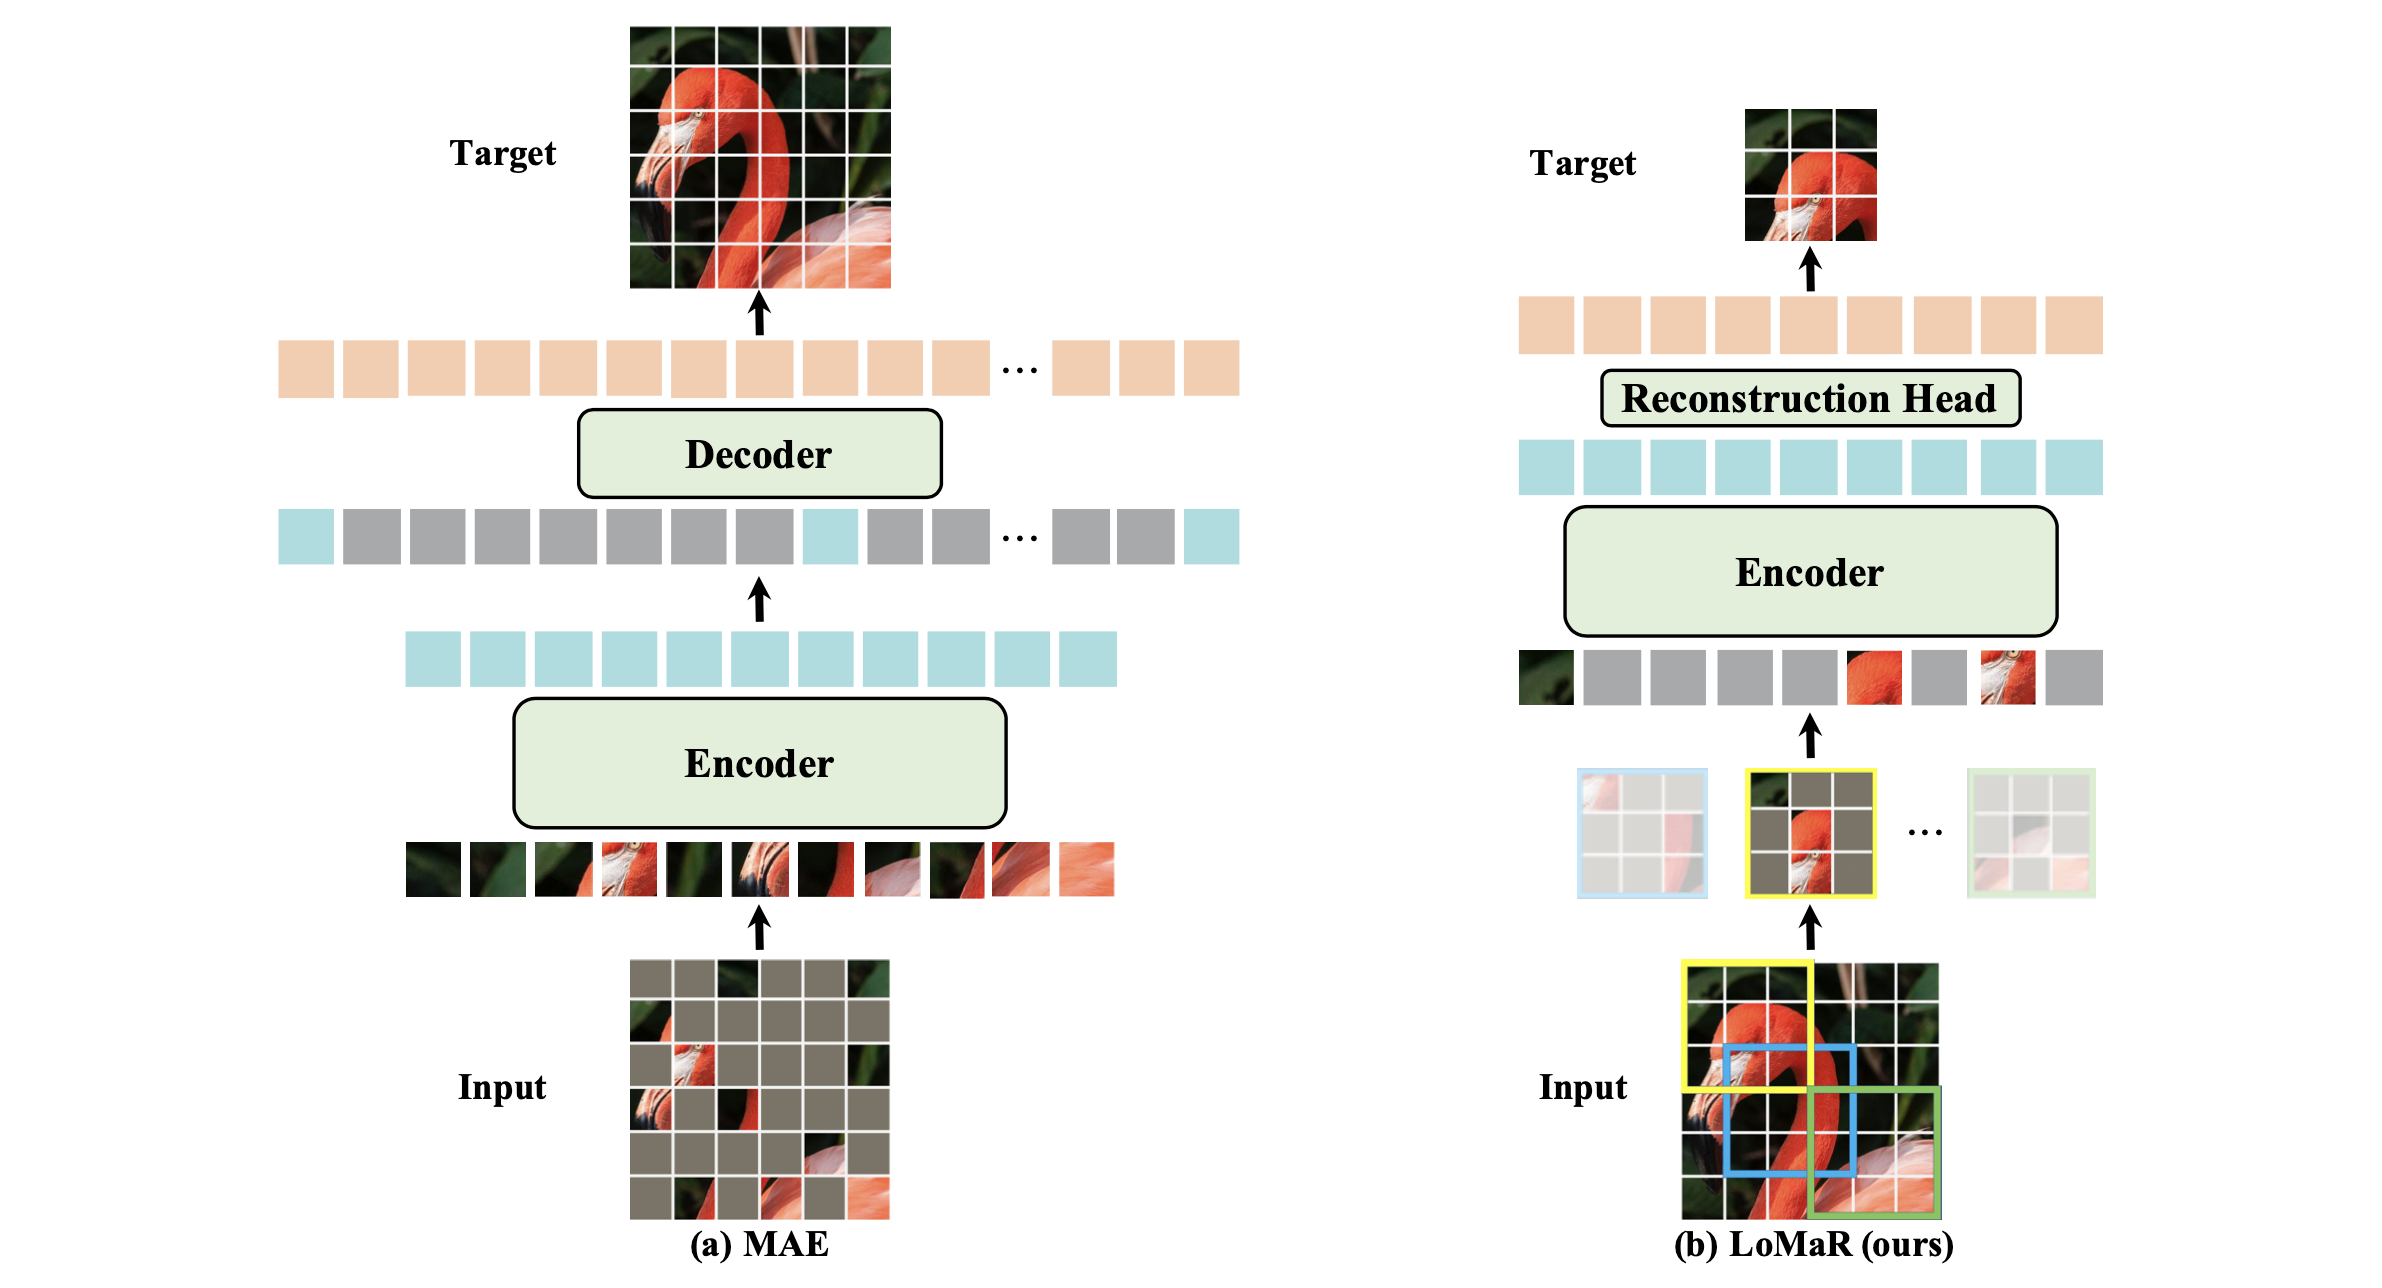
\includegraphics[width=\linewidth, trim={50mm 0 40mm 0}, clip]{assets/lomar.png}
    \caption{\label{fig:overview}The illustration of LoMaR.}
\end{figure}


{\small
\bibliographystyle{ieee}
\bibliography{egbib}
}

\end{document}
